
\documentclass{article}
\usepackage{graphicx} % for figures
\usepackage[margin=1.0in]{geometry} % 1-inch page margins
\usepackage{amsmath} % additional math symbols
\usepackage{hyperref} % embeding hypertext URLs (web links)
\usepackage{enumitem}
\renewcommand{\arraystretch}{2}

\begin{document}

\title{HW \#4: Football trajectory and Euler's Method}
\author{Aaron Deich}
%\date{24 September 2014} % if you want to set the date manually

\maketitle

Following the guidelines of the HW \#4 pseudocode, I wrote a Python program \texttt{balle.py} which computes and plots the trajectory of a football, both with the exact, analytic solution (in vacuum) and with Euler's method. If it's helpful, I'm storing my code in a GitHub repository at \url{https://github.com/adeich/Physics-240-Spring-2015/tree/master/HW4}

I first checked that my Euler's Method integrator agrees with the analytic vacuum trajectory by plotting both together:

\begin{figure}[h!]
  \caption{Vacuum trajectories of both analytic and Euler's method solutions. There appears to be fairly good agreement. Here, $v_0$ = 20 m/s and $\theta_0$ = 45 degrees.}
  \centering
    \includegraphics[width=1.1\textwidth]{20_45_no_air.png}
\end{figure}


(a) Football trajectory: Analytical vs Numerical (without air resistance)

\begin{figure}[h!]
  \caption{Here, $v_0$ = 20 m/s and $\theta_0$ = 45 degrees.}
  \centering
    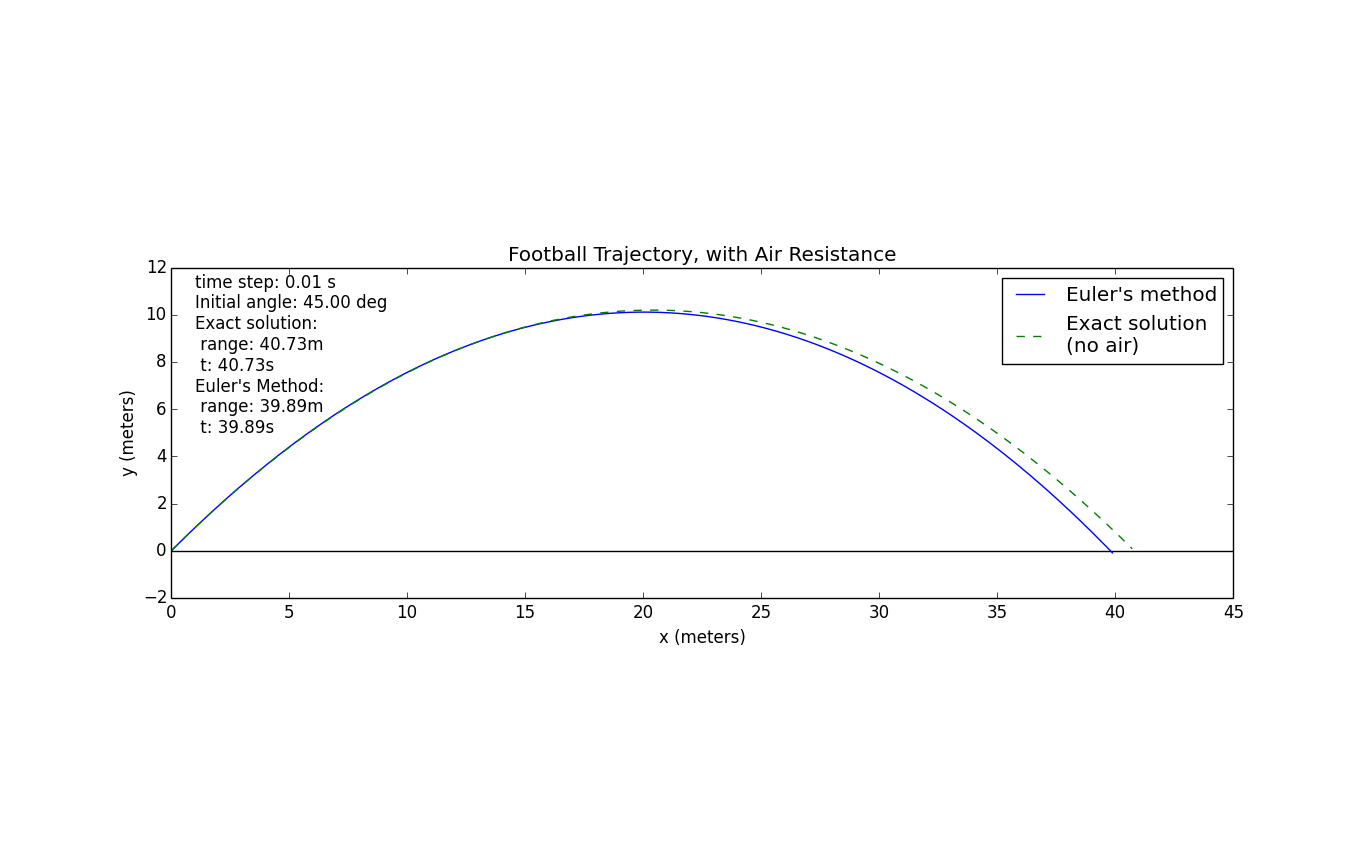
\includegraphics[width=1.1\textwidth]{20_45_yes_air.png}
\end{figure}

(b) 

\begin{figure}[h!]
  \caption{Vacuum trajectories of both analytic and Euler's method solutions. There appears to be fairly good agreement. Here, $v_0$ = 20 m/s and $\theta_0$ = 45 degrees.}
  \centering
    \includegraphics[width=1.1\textwidth]{30_30_yes_air.png}
\end{figure}

%\begin{tabular}{ l| l| l|  l| l| l }
%  Dwarf Galaxy    & RA              & DEC        & z              & i-band mag & petroRad   \\ \hline
%  CGCG 015-033 & 193.50786 &  -1.50834 & 0.003821 & 14.05          & 10.50 $\pm$ 0.146 
%\end{tabular}


%\begin{align*}
%\theta_{sep} &= \cos^{-1}(\sin(d1)\sin(d2) + \cos(d1)\cos(d2)\cos(r1 - r2)) \\
% &= 31.1 \mathrm{'}
%\end{align*}

\end{document}